In this chapter we present our results in chronological order. Many of the results 
are found based on earlier results, so we find it natural to include some amount 
of discussion of the results as they are presented to be able to argue for why we 
approach the problem the way we do further down.
\section{Feature reduction}
Note that when doing model selection we do not look at test set performance, only 
performance on the cross validated train set.
\begin{table}
    \begin{adjustbox}{width=\textwidth}
    \begin{tabular}{lr}
\toprule
{} &     Coeff \\
\midrule
Q95                   &  1.211018 \\
elev\_50               &  0.464968 \\
conductivity\_cosby\_50 &  0.443736 \\
intercept             &  0.443277 \\
porosity\_cosby\_50     &  0.409635 \\
conductivity\_hypres\_5 &  0.257509 \\
high\_prec\_dur         &  0.211253 \\
gauge\_easting         & -0.211231 \\
tawc                  & -0.326509 \\
elev\_max              & -0.349975 \\
conductivity\_cosby\_5  & -0.351292 \\
baseflow\_index\_ceh    & -0.417237 \\
bares\_perc            & -0.463398 \\
elev\_10               & -0.496951 \\
conductivity\_cosby\_95 & -0.839606 \\
porosity\_hypres\_5     & -1.030274 \\
low\_prec\_freq         & -1.055273 \\
dwood\_perc            & -1.288324 \\
p\_mean                & -2.015090 \\
ewood\_perc            & -2.146395 \\
urban\_perc            & -2.332153 \\
shrub\_perc            & -3.735298 \\
grass\_perc            & -4.010000 \\
crop\_perc             & -4.868455 \\
\bottomrule
\end{tabular}


    \end{adjustbox}
    \caption{Table for attempt at linear regression. This model is fit on the static
    features as input values, and the NSE of an LSTM trained without static features
    for each basin in the validation set. The $R^2$ score of this model is $\approx 0.5$}
    \label{linreg_no_static_table}
\end{table}
In table \ref{linreg_no_static_table} we can see that our linear regression used to model 
the relationship between NSE value of models and static features has decided that 
several features are important. All these coefficients have a p-value $<0.5$. The 
problem with this model was that it achieved an $R^2$ score of $\approx 0.5$, meaning 
it does not actually explain the relationship well. We therefore choose to change 
strategy for feature selection. 
\begin{figure}
    \includegraphics{{correlation_reduction/all_features/corr_and_dendrogram}.pdf}
    \caption{The Pearson correlation matrix and the corresponding hierarchial
    cluster of the training set before removing correlated features. The process
    of creating the dendrogrogram is described in chapter \ref{Feature selection}. 
    For readability's sake we cannot include every label in the correlation matrix.}
    \label{corr_matrix_full}
\end{figure}

\begin{figure}
    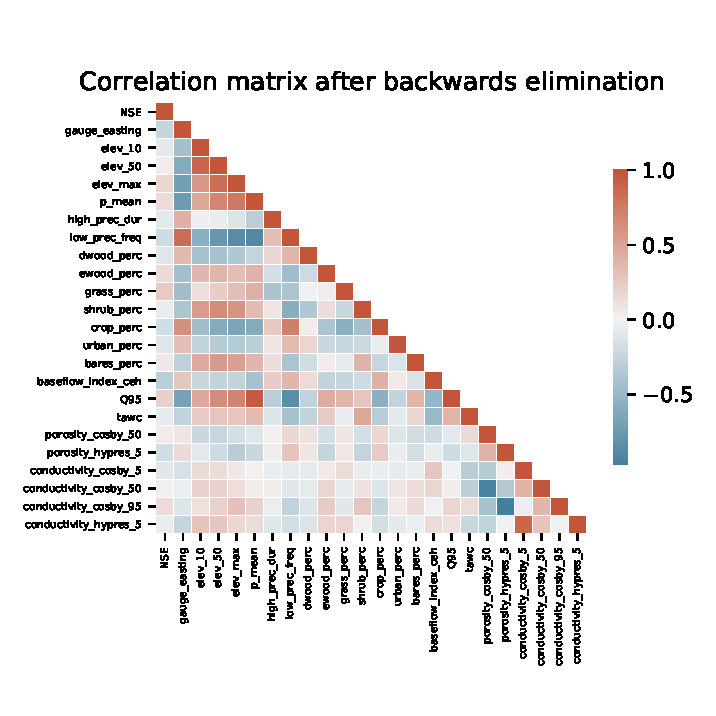
\includegraphics{reduced_matrix.pdf}
    \caption{Correlation matrix after backward selection}
    \label{corr_matrix_reduced}
\end{figure}

\subsection{Performance of full model}
\begin{figure}
%\includegraphics[scale=1]{{permutation/all_features_cv/histogram_all}.pdf}
    \includegraphics{{figures/permutation/all_features_cv/histogram_all}.pdf}
\caption{The two most important (above) and least important (below) features according 
to the permutation test}
\label{Hist all}
\end{figure}
